\documentclass[titlepage, letterpaper, fleqn]{article}
\usepackage[utf8]{inputenc}
\usepackage{fancyhdr} % fancy headers, of course!
\usepackage{amsmath} % what do you think?
\usepackage{amsthm} % theorems!
\usepackage{extramarks} % more cute things
\usepackage{enumitem} % i'm not sure...
\usepackage{multicol} % multicolumn...?
\usepackage{amssymb} % more symbols
\usepackage{MnSymbol} % moar symbols?
\usepackage{booktabs} % cool looking tables
\usepackage{tikz} %venn and shizzle
\usepackage{tikz-qtree-compat} %tableaux
\usepackage{lipsum} %lorem ipsum dolor sit amet f u
\usepackage{mathrsfs} %math script for calligraphic scripting, I GUESS

\topmargin=-0.45in
\evensidemargin=0in
\oddsidemargin=0in
\textwidth=6.5in
\textheight=9.0in
\headsep=0.25in


%
% You should change this things~
%

\newcommand{\mahteacher}{Dr. Viacheslav Kalashnikov}
\newcommand{\mahclass}{Applied Mathematics}
\newcommand{\mahtitle}{Topic II - Activity 10}
\newcommand{\mahdate}{October 11, 2016}
\newcommand{\spacepls}{\vspace{5mm}}
\newcommand{\until}{\mathscr{U}}
\renewcommand\qedsymbol{\(\blacksquare\)}

%
% Header markings
%

\pagestyle{fancy}
\lhead{1170065 - Xavier Sánchez}
\chead{}
\rhead{}
\lfoot{}
\rfoot{}


\renewcommand\headrulewidth{0.4pt}
\renewcommand\footrulewidth{0.4pt}

\setlength\parindent{0pt}


%
% Create Problem Sections (stolen directly from jdavis/latex-homework-template @ github!)
%

\newcommand{\enterProblemHeader}[1]{
\nobreak\extramarks{}{Problem \arabic{#1} continued on next page\ldots}\nobreak{}
\nobreak\extramarks{Problem \arabic{#1} (continued)}{Problem \arabic{#1} continued on next page\ldots}\nobreak{}
}

\newcommand{\exitProblemHeader}[1]{
\nobreak\extramarks{Problem \arabic{#1} (continued)}{Problem \arabic{#1} continued on next page\ldots}\nobreak{}
\stepcounter{#1}
\nobreak\extramarks{Problem \arabic{#1}}{}\nobreak{}
}

\setcounter{secnumdepth}{0}
\newcounter{partCounter}
\newcounter{homeworkProblemCounter}
\setcounter{homeworkProblemCounter}{1}
\nobreak\extramarks{Exercise \arabic{homeworkProblemCounter}}{}\nobreak{}

% Alias for the Solution section header
\newcommand{\solution}{\textbf{\Large Solution}}

%Alias for the new step section
\newcommand{\steppy}[1]{\textbf{\large #1}}

%
% Homework Problem Environment
%
% This environment takes an optional argument. When given, it will adjust the
% problem counter. This is useful for when the problems given for your
% assignment aren't sequential. See the last 3 problems of this template for an
% example.
%
\newenvironment{homeworkProblem}[1][-1]{
\ifnum#1>0
\setcounter{homeworkProblemCounter}{#1}
\fi
\section{Exercise \arabic{homeworkProblemCounter}}
\setcounter{partCounter}{1}
\enterProblemHeader{homeworkProblemCounter}
}{
\exitProblemHeader{homeworkProblemCounter}
}

%
% My actual info
%

\title{
\vspace{1in}
\textbf{Tecnológico de Monterrey} \\
\vspace{0.5in}
\textmd{\mahclass} \\
\large{\textit{\mahteacher}} \\
\vspace{0.5in}
\textsc{\mahtitle}\\
\textsc{2.4.1 Linear Temporal Logic}\\
\textsc{2.4.2 Linear Temporal Logic}\\
\textsc{2.4.3 Linear Temporal Logic}\\
\textsc{2.4.4 Linear Temporal Logic}\\
\textsc{2.4.5 Linear Temporal Logic}\\
\textsc{2.5.1 Computational Tree Logic}\\
\textsc{2.5.2 Computational Tree Logic}\\
\textsc{2.6.1 Computational Tree Logic*}\\
\author{01170065  - MIT \\
Xavier Fernando Cuauhtémoc Sánchez Díaz \\
\texttt{xavier.sanchezdz@gmail.com}}
\date{\mahdate}
}

\begin{document}

\begin{titlepage}
\maketitle
\end{titlepage}

%
% Actual document starts here~
%

\section{Exercise 2.4.1}

{\large \textbf{a)} Prove \(\models \neg \Diamond \neg p \implies \Box p\) (the converse direction of Theorem 13.14 in Ben-Ari, M.).}

\spacepls

\begin{proof}
By duality of operators, \(\neg \Diamond \neg p\) can be expressed as \(\Box p\), therefore, the formula \(\neg \Diamond \neg p \implies \Box p\) is valid.
\end{proof}

\section{Exercise 2.4.2}

{\large \textbf{a)} Prove Theorem 13.34 from Ben-Ari, M., \(\models (\Diamond \Box p \wedge \Box \Diamond q) \implies \Box \Diamond(p \wedge q).\)}

\spacepls

\begin{proof}
\begin{align*}
& (\Diamond \Box p \wedge \Box \Diamond q) \implies \Box \Diamond (p \wedge q) = &
\\ & = (\Box \Diamond p \wedge \Box \Diamond q) \implies \Box \Diamond (p \wedge q) & \tag*{Commutativity of $\Diamond \Box$}
\\ & = \Box (\Diamond p \wedge \Diamond q) \implies \Box \Diamond (p \wedge q) & \tag*{$\Box$ distributes over $\wedge$}
\\ & = \Box (\Diamond p \wedge \Diamond q) \implies \Box (\Diamond p \wedge \Diamond q) & \tag*{$\Diamond$ distributes over $\wedge$ in this direction}
\end{align*}
\end{proof}

\section{Exercise 2.4.3}

{\large \textbf{a)} Construct a tableau and find a model for the negation of \(\Box \Diamond p \implies \Diamond \Box p\).}

\spacepls

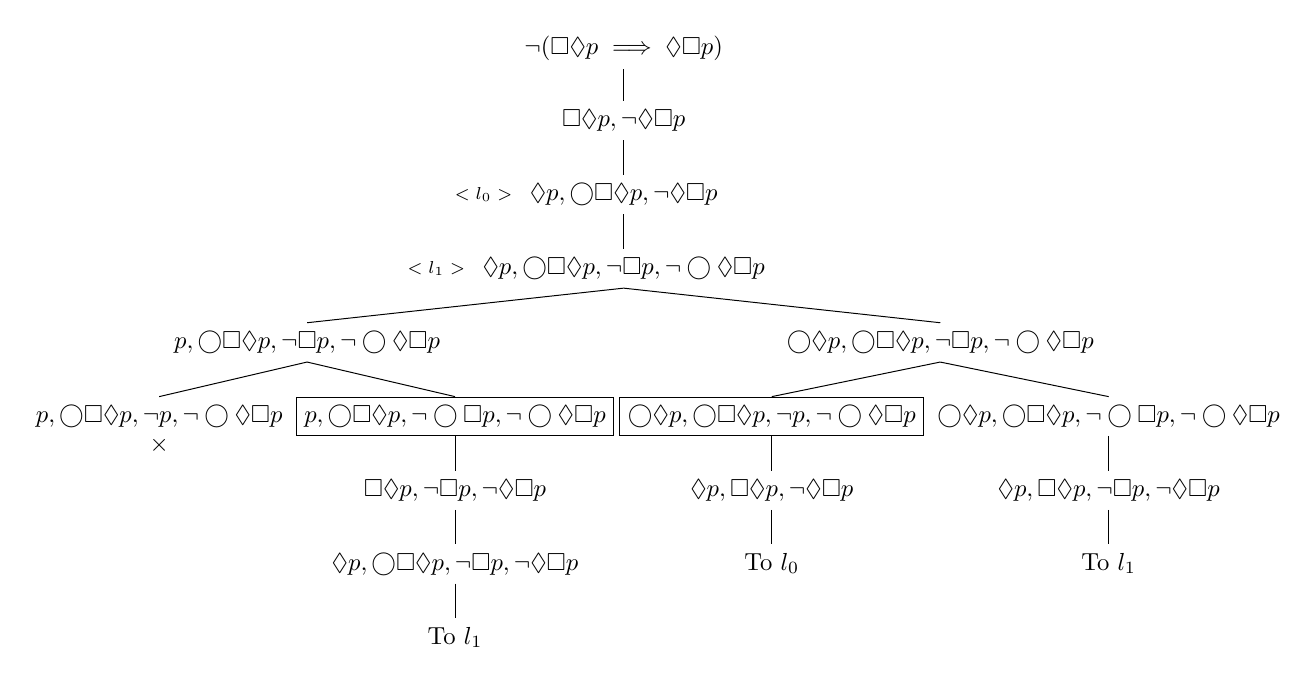
\begin{tikzpicture}[scale=0.89]
\tikzset{every tree node/.style={align=center,anchor=north}}
\tikzset{grow'=down}
\Tree [.{$\neg (\Box \Diamond p \implies \Diamond \Box p)$} 
[.{$\Box \Diamond p, \neg \Diamond \Box p$} 
[.\node[label=left:{\scriptsize $<l_0>$}]{$\Diamond p, \bigcirc \Box \Diamond p, \neg \Diamond \Box p$}; 
[.\node[label=left:{\scriptsize $<l_1>$}]{$\Diamond p, \bigcirc \Box \Diamond p, \neg \Box p, \neg \bigcirc \Diamond \Box p$}; 
[.{$\bigcirc \Diamond p, \bigcirc \Box \Diamond p, \neg \Box p, \neg \bigcirc \Diamond \Box p$} 
[.{$\bigcirc \Diamond p , \bigcirc \Box \Diamond p, \neg \bigcirc \Box p, \neg \bigcirc \Diamond \Box p$} 
[.{$\Diamond p, \Box \Diamond p, \neg \Box p, \neg \Diamond \Box p$} 
[.{To $l_1$} ] ] ] 
[.\node[draw]{$\bigcirc \Diamond p , \bigcirc \Box \Diamond p, \neg p, \neg \bigcirc \Diamond \Box p$}; 
[.{$\Diamond p, \Box \Diamond p, \neg \Diamond \Box p$} 
[.{To $l_0$} ] ] ] ] 
[.{$p, \bigcirc \Box \Diamond p, \neg \Box p, \neg \bigcirc \Diamond \Box p$} 
[.\node[draw]{$p, \bigcirc \Box \Diamond p, \neg \bigcirc \Box p, \neg \bigcirc \Diamond \Box p$}; 
[.{$\Box \Diamond p, \neg \Box p, \neg \Diamond \Box p$} 
[.{$\Diamond p, \bigcirc \Box \Diamond p, \neg \Box p, \neg \Diamond \Box p$} 
[.{To $l_1$} ] ] ] ] 
[.{$p, \bigcirc \Box \Diamond p, \neg p, \neg \bigcirc \Diamond \Box p$}\\{$\times$} ] ] ] ] ] ]
\end{tikzpicture}

\begin{proof}
Since the tableau for the negation of \(\Box \Diamond p \implies \Diamond \Box p\) shows a closed branch but many looped branches, it is then satisfiable.
\end{proof}

\pagebreak

\section{Exercise 2.4.4}

{\large \textbf{a)} Prove that a linear interpretation is characterized by \(\bigcirc A \iff \neg \bigcirc \neg A\) (Theorem 13.25 from Ben-Ari, M.).}

\spacepls

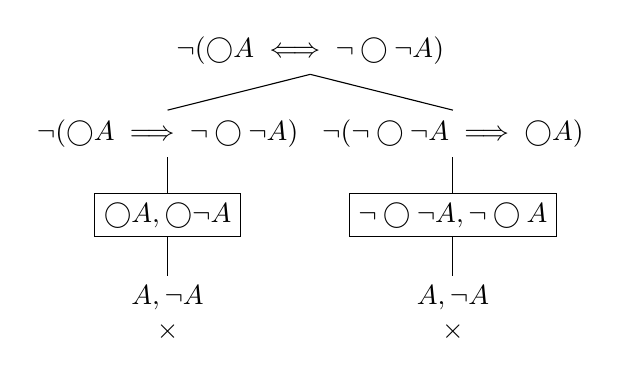
\begin{tikzpicture}
\tikzset{every tree node/.style={align=center,anchor=north}}
\tikzset{grow'=down}
\Tree [.{$\neg(\bigcirc A \iff \neg \bigcirc \neg A)$}
[.{$\neg (\neg \bigcirc \neg A \implies \bigcirc A)$} 
[. \node[draw]{$\neg \bigcirc \neg A, \neg \bigcirc A$};
[.{$A, \neg A$}\\{$\times$} ] ] ] 
[.{$\neg (\bigcirc A \implies \neg \bigcirc \neg A)$} 
[. \node[draw]{$\bigcirc A, \bigcirc \neg A$};
[.{$A, \neg A$}\\{$\times$} ] ] ] ]
\end{tikzpicture}

\begin{proof}
Since the converse of the double implication is marked as unsatisfiable in the LTL tableau,
then it means the \(\bigcirc A\) is equivalent to \(\neg \bigcirc \neg A\) for LTL formulas.
\end{proof}

\section{Exercise 2.4.5}

{\large \textbf{a)} Check if the formula \(\bigcirc \bigcirc A \implies \bigcirc A\) is satisfiable, and/or valid.}

\spacepls

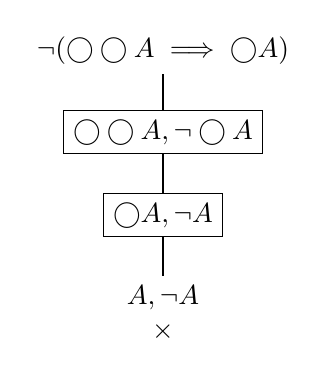
\begin{tikzpicture}
\tikzset{every tree node/.style={align=center,anchor=north}}
\tikzset{grow'=down}
\Tree [.{$\neg(\bigcirc \bigcirc A \implies \bigcirc A)$}
[. \node[draw]{$\bigcirc \bigcirc A, \neg \bigcirc A$}; 
[. \node[draw]{$\bigcirc A, \neg A$}; {$A, \neg A$}\\{$\times$} ] ] ]
\end{tikzpicture}

\begin{proof}
Since the tableau ends with its only branch as closed, then the formula \(\bigcirc \bigcirc A \implies \bigcirc A\) is valid.
\end{proof}

{\large \textbf{b)} Check if the formula \(\bigcirc (A \vee \Diamond A) \implies \Diamond A\) is satisfiable, and/or valid.}

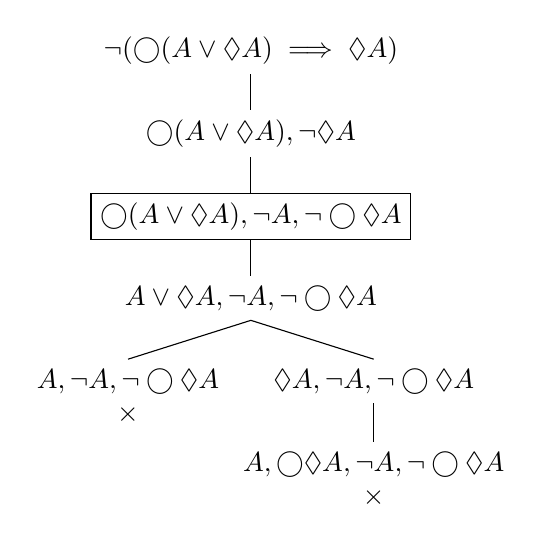
\begin{tikzpicture}
\tikzset{every tree node/.style={align=center,anchor=north}}
\tikzset{grow'=down}
\Tree [.{$\neg(\bigcirc(A \vee \Diamond A) \implies \Diamond A)$} 
[.{$\bigcirc(A \vee \Diamond A), \neg \Diamond A$} 
[. \node[draw]{$\bigcirc (A \vee \Diamond A), \neg A, \neg \bigcirc \Diamond A$}; 
[.{$A \vee \Diamond A, \neg A, \neg \bigcirc \Diamond A$} 
[.{$\Diamond A, \neg A, \neg \bigcirc \Diamond A$} {$A, \bigcirc \Diamond A, \neg A, \neg \bigcirc \Diamond A$}\\{$\times$} ] 
[.{$A, \neg A, \neg \bigcirc \Diamond A$}\\{$\times$} ] ] ] ] ]
\end{tikzpicture}

\begin{proof}
Since all branches in the tableau are closed, the formula \(\bigcirc (A \vee \Diamond A) \implies \Diamond A\) is valid.
\end{proof}

{\large \textbf{c)} Check if the formula \(\Box A \implies \neg \bigcirc (\neg A \wedge \Box \neg A)\) is satisfiable, and/or valid.}

\spacepls

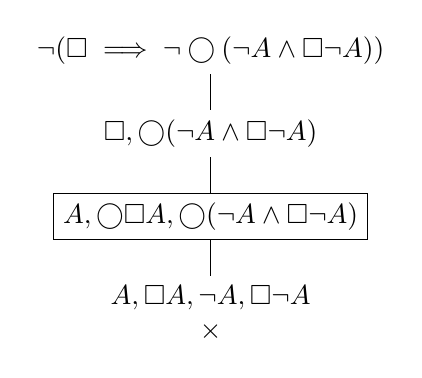
\begin{tikzpicture}
\tikzset{every tree node/.style={align=center,anchor=north}}
\tikzset{grow'=down}
\Tree [.{$\neg(\Box \implies \neg \bigcirc (\neg A \wedge \Box \neg A))$} 
[.{$\Box, \bigcirc(\neg A \wedge \Box \neg A)$} 
[.\node[draw]{$A, \bigcirc \Box A, \bigcirc (\neg A \wedge \Box \neg A)$}; 
[.{$A, \Box A, \neg A, \Box \neg A$}\\{$\times$} ] ] ] ]
\end{tikzpicture}

\begin{proof}
Since the only branch in the tableau is closed, \(\Box A \implies \neg \bigcirc (\neg A \wedge \Box \neg A)\) is a valid formula.
\end{proof}

{\large \textbf{d)} Check if the formula \((\Box A)\until(\Diamond B) \implies \Box(A \until \Box B)\) is satisfiable, and/or valid.}

\spacepls

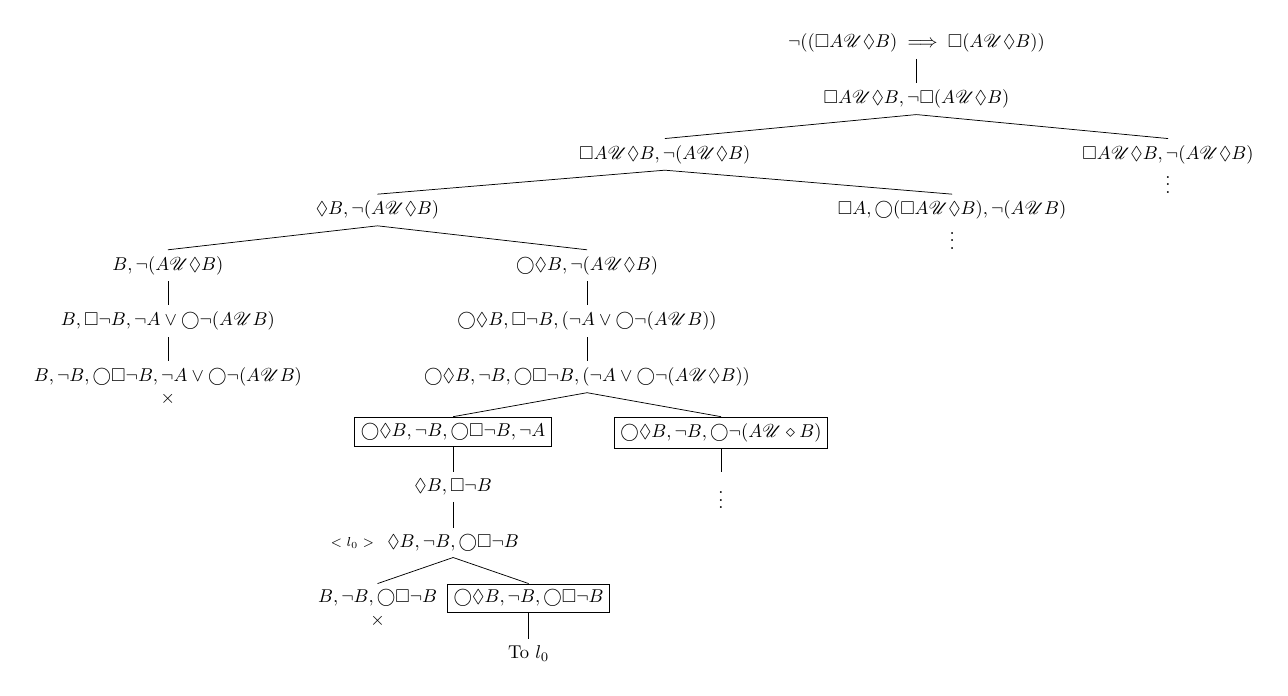
\begin{tikzpicture}[scale=0.67]
\tikzset{every tree node/.style={align=center,anchor=north}}
\tikzset{grow'=down}
\Tree [.{$\neg ((\Box A \until \Diamond B) \implies \Box (A \until \Diamond B))$} [.{$\Box A \until \Diamond B, \neg \Box (A \until \Diamond B)$} [.{$\Box A \until \Diamond B, \neg (A \until \Diamond B)$}\\{$\vdots$} ] [.{$\Box A \until \Diamond B, \neg (A \until \Diamond B)$} [.{$\Box A, \bigcirc(\Box A \until \Diamond B), \neg (A \until B)$}\\{$\vdots$} ] [.{$\Diamond B, \neg (A \until \Diamond B)$} [.{$\bigcirc \Diamond B, \neg (A \until \Diamond B)$} [.{$\bigcirc \Diamond B, \Box \neg B, (\neg A \vee \bigcirc \neg (A \until B))$} [.{$\bigcirc \Diamond B, \neg B, \bigcirc \Box \neg B, (\neg A \vee \bigcirc \neg (A \until \Diamond B))$} [.\node[draw]{$\bigcirc \Diamond B, \neg B, \bigcirc \neg(A \until \diamond B)$};\\{$\vdots$} ] [.\node[draw]{$\bigcirc \Diamond B, \neg B, \bigcirc \Box \neg B, \neg A$}; [.{$\Diamond B, \Box \neg B$} [.\node[label=left:{\scriptsize $<l_0>$}]{$\Diamond B, \neg B, \bigcirc \Box \neg B$}; [.\node[draw]{$\bigcirc \Diamond B, \neg B, \bigcirc \Box \neg B$}; [.{To $l_0$} ] ] [.{$B, \neg B, \bigcirc \Box \neg B$}\\{$\times$} ] ] ] ] ] ] ] [.{$B, \neg (A \until \Diamond B)$} [.{$B, \Box \neg B, \neg A \vee \bigcirc \neg(A \until B)$} [.{$B, \neg B, \bigcirc \Box \neg B, \neg A \vee \bigcirc \neg(A \until B)$}\\{$\times$} ] ] ] ] ] ] ]
\end{tikzpicture}

\begin{proof}
As there is at least one branch that loops and some branches that are closed, \((\Box A)\until(\Diamond B) \implies \Box(A \until \Box B)\)
is not valid but satisfiable.
\end{proof}

\pagebreak

{\large \textbf{e)} Check if the formula \(\Diamond B \implies (A \until B)\) is satisfiable, and/or valid.}

\spacepls

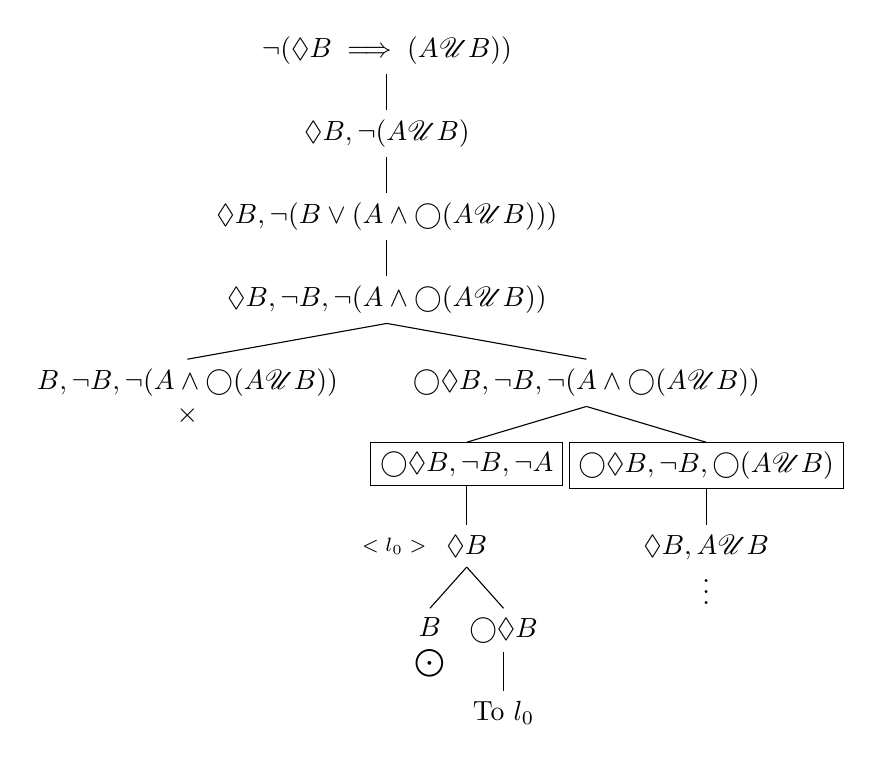
\begin{tikzpicture}
\tikzset{every tree node/.style={align=center,anchor=north, }}
\tikzset{grow'=down}
\Tree [.{$\neg(\Diamond B \implies (A \until B))$} 
[.{$\Diamond B, \neg(A \until B)$} 
[.{$\Diamond B, \neg(B \vee (A \wedge \bigcirc(A \until B)))$} 
[.{$\Diamond B, \neg B, \neg(A \wedge \bigcirc(A \until B))$} 
[.{$\bigcirc \Diamond B, \neg B, \neg(A \wedge \bigcirc(A \until B))$} 
[.\node[draw]{$\bigcirc \Diamond B, \neg B, \bigcirc(A \until B)$}; 
[.{$\Diamond B, A \until B$}\\{$\vdots$} ] ]
[.\node[draw]{$\bigcirc \Diamond B, \neg B, \neg A$}; 
[.\node[label={left:{\scriptsize $<l_0>$}}]{$\Diamond B$}; 
[.{$\bigcirc \Diamond B$} {To $l_0$} ] 
[.{$B$\\{$\bigodot$}} ] ] ] ] 
[.{$B, \neg B, \neg(A \wedge \bigcirc(A \until B))$}\\{$\times$} ] ] ] ] ]
\end{tikzpicture}

\begin{proof}
As there is a loop and an open branch in the tableau, the formula \(\Diamond B \implies (A \until B)\) is not valid.
\end{proof}

\section{Exercise 2.5.1}

{\large \textbf{a)} Is the following assertion correct? Provide a proof or a counterexample.

If \(s \models \exists A\), then \(s \models \forall A\).}

\spacepls

This is not correct.
\begin{proof}
Let \(e_1\) be an edge between \(s\) and \(s'\), and \(v_{\mathscr{I}_{s'}}(A) = T\).

Now assume \(e_2\) is an edge between \(s\) and \(s''\), and that \(v_{\mathscr{I}_{s''}}(A) = F\).

Therefore, it exists a path where there's a state \(s'\) where \(A\) is true, but not all paths of \(s\) lead to states where \(A\) is true.
\end{proof}

{\large \textbf{b)} Is the following assertion correct? Provide a proof or a counterexample.

If \(s \models \forall A\), then \(s \models \exists A\).}

\spacepls

This is correct.

\begin{proof}
Let \(e_1\) and \(e_2\) be edges connecting \(s\) to \(s'\) and \(s''\) respectively, and that the premise \(s \models \forall A\) is correct, so that \(v_{\mathscr{I}_{s'}}(A) = T, v_{\mathscr{I}_{s''}}(A) = T\).

Therefore, there exists a path of \(s\) that leads to a state in which \(A\) is true.
\end{proof}

\pagebreak

{\large \textbf{c)} Is the following assertion correct? Provide a proof or a counterexample.

If \(s \models \forall \Diamond A \vee \forall \Diamond B\), then \(s \models \forall \Diamond (A \vee B)\).}

\spacepls

This is correct.

\begin{proof}
Let  the premise \(s \models \forall \Diamond A \vee \forall \Diamond B\) be true. For the premise to be true, either there are some states \(s', \, \dots , \, s^n\) in all paths connected to \(s\) in which A is true, or either there are some states \(s_1, \, \dots , \, s_m\) in all paths connected to \(s\) where \(B\) is true.

This means that all paths connected to \(s\) have some states where either \(A\) or \(B\) is true, and therefore, the assertion holds.
\end{proof}

However, the converse direction does not hold, as is shown in the next exercise.

\spacepls

{\large \textbf{d)} Is the following assertion correct? Provide a proof or a counterexample.

If \(s \models \forall \Diamond(A \vee B)\), then \(s \models \forall \Diamond A \vee \Diamond B\).}

\spacepls

This is not correct. Consider the following counterexample.

\begin{proof}
Let \(e_1\) and \(e_2\) be edges connecting \(s\) to \(s'\) and \(s''\) respectively, and that the premise is correct, so that \(v_{\mathscr{I}_{s'}}(A) = T, v_{\mathscr{I}_{s'}}(B) = F, v_{\mathscr{I}_{s''}}(A) = F, v_{\mathscr{I}_{s''}}(B) = T\).

So it is true that all paths have at least one state in which either A or B is true, but conversely, not all paths lead to an \(A\) neither all paths lead to a \(B\).
Therefore this implication is not correct.
\end{proof}

{\large \textbf{e)} Is the following assertion correct? Provide a proof or a counterexample.

If \(s \models \forall (A \until B)\), then \(s \models \neg (\exists (\neg B \until(\neg A \wedge \neg B)) \vee \exists \Diamond \neg B)\).}

\spacepls

This is correct.

\begin{proof}
\begin{align*}
& \forall (A \until B) \implies \neg (\exists (\neg B \until(\neg A \wedge \neg B)) \vee \exists \Diamond \neg B) =
\\ & = \neg \exists (\neg B \until(\neg A \wedge \neg B)) \wedge \exists \Box \neg B & \tag*{Equivalence of $A \until B$}
\\ & = \neg (\exists (B \until(\neg A \wedge \neg B)) \vee \exists \Diamond \neg B) & \tag*{de Morgan}
\end{align*}
\end{proof}

\section{Exercise 2.5.2}

{\large \textbf{a)} Let \(\Phi\) and \(\Psi\) be arbitrary CTL formulae. Is the following equivalence correct?
\[\exists \bigcirc \exists \Diamond \Phi \equiv \exists \Diamond \exists \bigcirc \Phi\]}

This is correct.

\begin{proof}
Let the LHS of the equivalence be true.
This means that there exists at least one path in which one of the next states of the current state \(s\) has at least one path with a state where \(\Phi\) is true.

Now, let the RHS of the equivalence be true.
This would mean that exists at least one path in which one of its states has at least one next state in which \(\Phi\) is true.

Let \(s^i\) be a state where \(\Phi\) holds and that is somehow connected to the current state \(s\).
Since each state \(s^i\) has a previous state \(s^{i-1}\), then the RHS holds for \(s^{i-1}\). Since \(s\) is connected to \(s^1\), and \(s^1\) is connected to \(s^i\), then the LHS also holds.

Therefore, the equivalence is correct.
\end{proof}

{\large \textbf{b)} Let \(\Phi\) and \(\Psi\) be arbitrary CTL formulae. Is the following equivalence correct?
\[\forall \bigcirc \forall \Box \Phi \equiv \forall \Box \forall \bigcirc \Phi\]}

This equivalence is correct.

\begin{proof}
Let us consider the semantics of the LHS, assuming it holds true.
LHS implies that all next states \(s'\) in all paths from the current state \(s\) have all states \(s'',\, \dots,\, s^n\)in all their paths with \(\Phi\) as true. This means that \(\Phi\) should be true for all states in all branches of all \(s''\) next states of \(s^i\), from \(i=1\) to \(i=n-1\).

Now let's consider the RHS and assuming it's true.
RHS implies that all states \(s', \, \dots , \, s^n\) from all paths from the current state \(s\) have a next state \(s^{i+1}\) in all their paths such that \(\Phi\) is true. This means that \(\Phi\) should be true for all the next states in all branches of \(s^{i+1}\) such that \(1<i<n\).

Hence, the equivalence is correct. This also proves that \(\forall \bigcirc\) and \(\forall \Box\) are commutative.

\end{proof}

{\large \textbf{c)} Let \(\Phi\) and \(\Psi\) be arbitrary CTL formulae. Is the following equivalence correct?
\[\exists \bigcirc \exists \Box \Phi \equiv \exists \Box \exists \bigcirc \Phi\]}

This equivalence is not correct.

\begin{proof}
Considering the semantics of the LHS of the equivalence, we have that there is at least one path of the current state \(s\) in which the next state \(s'\) has at least one path with all its states with \(\Phi\) as true.

Now let'sconsider the RHS, where we have that there is at least one path of the current state \(s\) in which all states have at least one path containing a next state \(s^{i+1}\) such that \(1<i<n\) where \(\Phi\) is true.

The LHS of the equivalence refers to one of the next states with a branch (at least one) with all states (many) where \(\Phi\) is true, while RHS mentions that there exists a branch in which all states (many) have a branch that has a next state (at least one) in which \(\Phi\) is true.
\end{proof}

{\large \textbf{d)} Let \(\Phi\) and \(\Psi\) be arbitrary CTL formulae. Is the following equivalence correct?
\[\forall \Box(\Phi \implies \Psi) \equiv (\exists \bigcirc \Phi \implies \exists \bigcirc \Psi)\]}

This equivalence is not correct. Consider the following counterexample:

\begin{proof}
Let \(\Phi \implies \Psi\) be true, so that all states from all branches in the LHS of the equivalence are true.

The RHS states that if there is at least one branch with a next state  in which \(\Phi\) is true, then there is at least one branch with a next state in which \(\Psi\) is true, but not necessarily the same.

Therefore, a state could have \(\Phi\) as true, but a false value for \(\Psi\).
\end{proof}

\pagebreak

\section{Exercise 2.6.1}

{\large \textbf{a)} Is this equivalence correct? Provide a proof or a counterexample.
\[\forall \bigcirc \forall \Box \Phi \equiv \forall \bigcirc \Box \Phi\]}

This equivalence is correct.

\begin{proof}
\begin{align*}
& \forall \bigcirc \forall \Box \Phi =
\\ & = \forall \bigcirc \Box \Phi & \tag*{Quantifier absorption}
\end{align*}
\begin{align*}
& \forall \bigcirc \Box \Phi =
\\ & = \forall \bigcirc \forall \Box \Phi & \tag*{Quantifier absorption}
\end{align*}
\end{proof}

{\large \textbf{b)} Is this equivalence correct? Provide a proof or a counterexample.
\[\exists \bigcirc \exists \Box \Phi \equiv \exists \bigcirc \Box \Phi\]}

This equivalence is not correct.

\begin{proof}
The LHS states that at least one of the next states of the branches of the current state \(s\), has at least one branch with all its states with \(\Phi\) as true.

The RHS, however, mentions that at least one of the next states of the branches of the current state \(s\) always yields \(\Phi\) as true.

For the RHS, consider a state \(s'\) with two edges \(e_1, e_2\) connecting to \(s'', s'''\) respectively. Since \(\Phi\) is always true in the future of \(s'\), then both \(s''\) and \(s'''\) should hold \(\Phi\).

However, it is not the case for the LHS, since it explicitly states that at one branch (at least) of the state \(s'\) always holds \(\Phi\) as true. Therefore, these formulas are semantically different.
\end{proof}

{\large \textbf{c)} Is this equivalence correct? Provide a proof or a counterexample.
\[\forall (\phi \wedge \psi) \equiv \forall \phi \wedge \forall \psi\]}

This is correct.

\begin{proof}
\begin{align*}
& \forall (\phi \wedge \psi) =
\\ & = \forall \phi \wedge \forall \psi & \tag*{$\forall$ distributes over $\wedge$ in both directions}
\end{align*}
\end{proof}

\pagebreak

{\large \textbf{d)} Is this equivalence correct? Provide a proof or a counterexample.
\[\exists (\phi \wedge \psi) \equiv \exists \phi \wedge \exists \psi\]}

This equivalence is not correct.

\begin{proof}
Since \(\exists\) distributes over \(\wedge\) in only one direction (\(\exists (\phi \wedge \psi) \implies \exists \phi \wedge \exists \psi\)) but not the other way around, this equivalence is incorrect.
\end{proof}

{\large \textbf{e)} Is this equivalence correct? Provide a proof or a counterexample.
\[\neg \forall(\phi \implies \psi) \equiv \exists (\phi \wedge \neg \psi)\]}

This equivalence is correct.

\begin{proof}
\begin{align*}
& \neg \forall(\phi \implies \psi) \equiv \exists (\phi \wedge \neg \psi) =
\\ & = \exists \neg (\phi \implies \psi) \equiv \exists (\phi \wedge \neg \psi) & \tag*{Duality of quantifiers}
\\ & = \exists \neg (\neg \phi \vee \psi) \equiv \exists (\phi \wedge \neg \psi) & \tag*{Material implication}
\\ & = \exists (\phi \wedge \neg \psi) \equiv \exists (\phi \wedge \neg \psi) & \tag*{de Morgan}
\end{align*}
\end{proof}

{\large \textbf{f)} Is this equivalence correct? Provide a proof or a counterexample.
\[\forall (\Diamond \Psi \wedge \Box \Phi) \equiv \forall \Diamond (\Psi \wedge \forall \Box \Phi) \wedge \forall \Box (\Phi \wedge \forall \Diamond \Psi)\]}

This equivalence is correct.

\begin{proof}
The LHS states that along all paths, \(\Psi\) is eventually true and \(\Phi\) is always true.

The RHS states the same in a bit different manner: along all paths there is at least one state in which \(\Psi\) is true and along all paths all states have \(\Phi\) as true. And that along all paths, all states have \(\Phi\) as true, and along all paths \(\Psi\) is eventually true.

This can be easily seen as the universal quantifier can be distributed over conjunction. And since LTL formulas (state formulas) are considered as always being quantified with \(\forall\).
\end{proof}
\end{document}